\chapter{Methodology}

%Algorithm training process:
%\begin{enumerate}
%\item Plants in the imagery will be localized with Faster R-CNN \cite{r-cnn} and cropped
%\item Localized plants will be associated with plant ID
%\item Cropped images will be used as training data, where targets are the plant health indicators
%\end{enumerate}

\section{Dataset Creation}
In this section, we go over the instruments and the process that we used to create the dataset.

\subsection{Instruments}
For the UAV, we utilized two different systems: Aibotix's Aibot X6 and PrecisionHawk's Lancaster 5 as pictured in Figures \ref{aibotx6} and \ref{lancaster5}. The Aibot X6 is a multirotor UAV equipped with a Headwall Nano-Hyperspec sensor. The Lancaster 5 is a fixed-wing UAV equipped with INSERT SENSOR HERE AND CAPABILITIES.


\begin{figure}
    \centering
    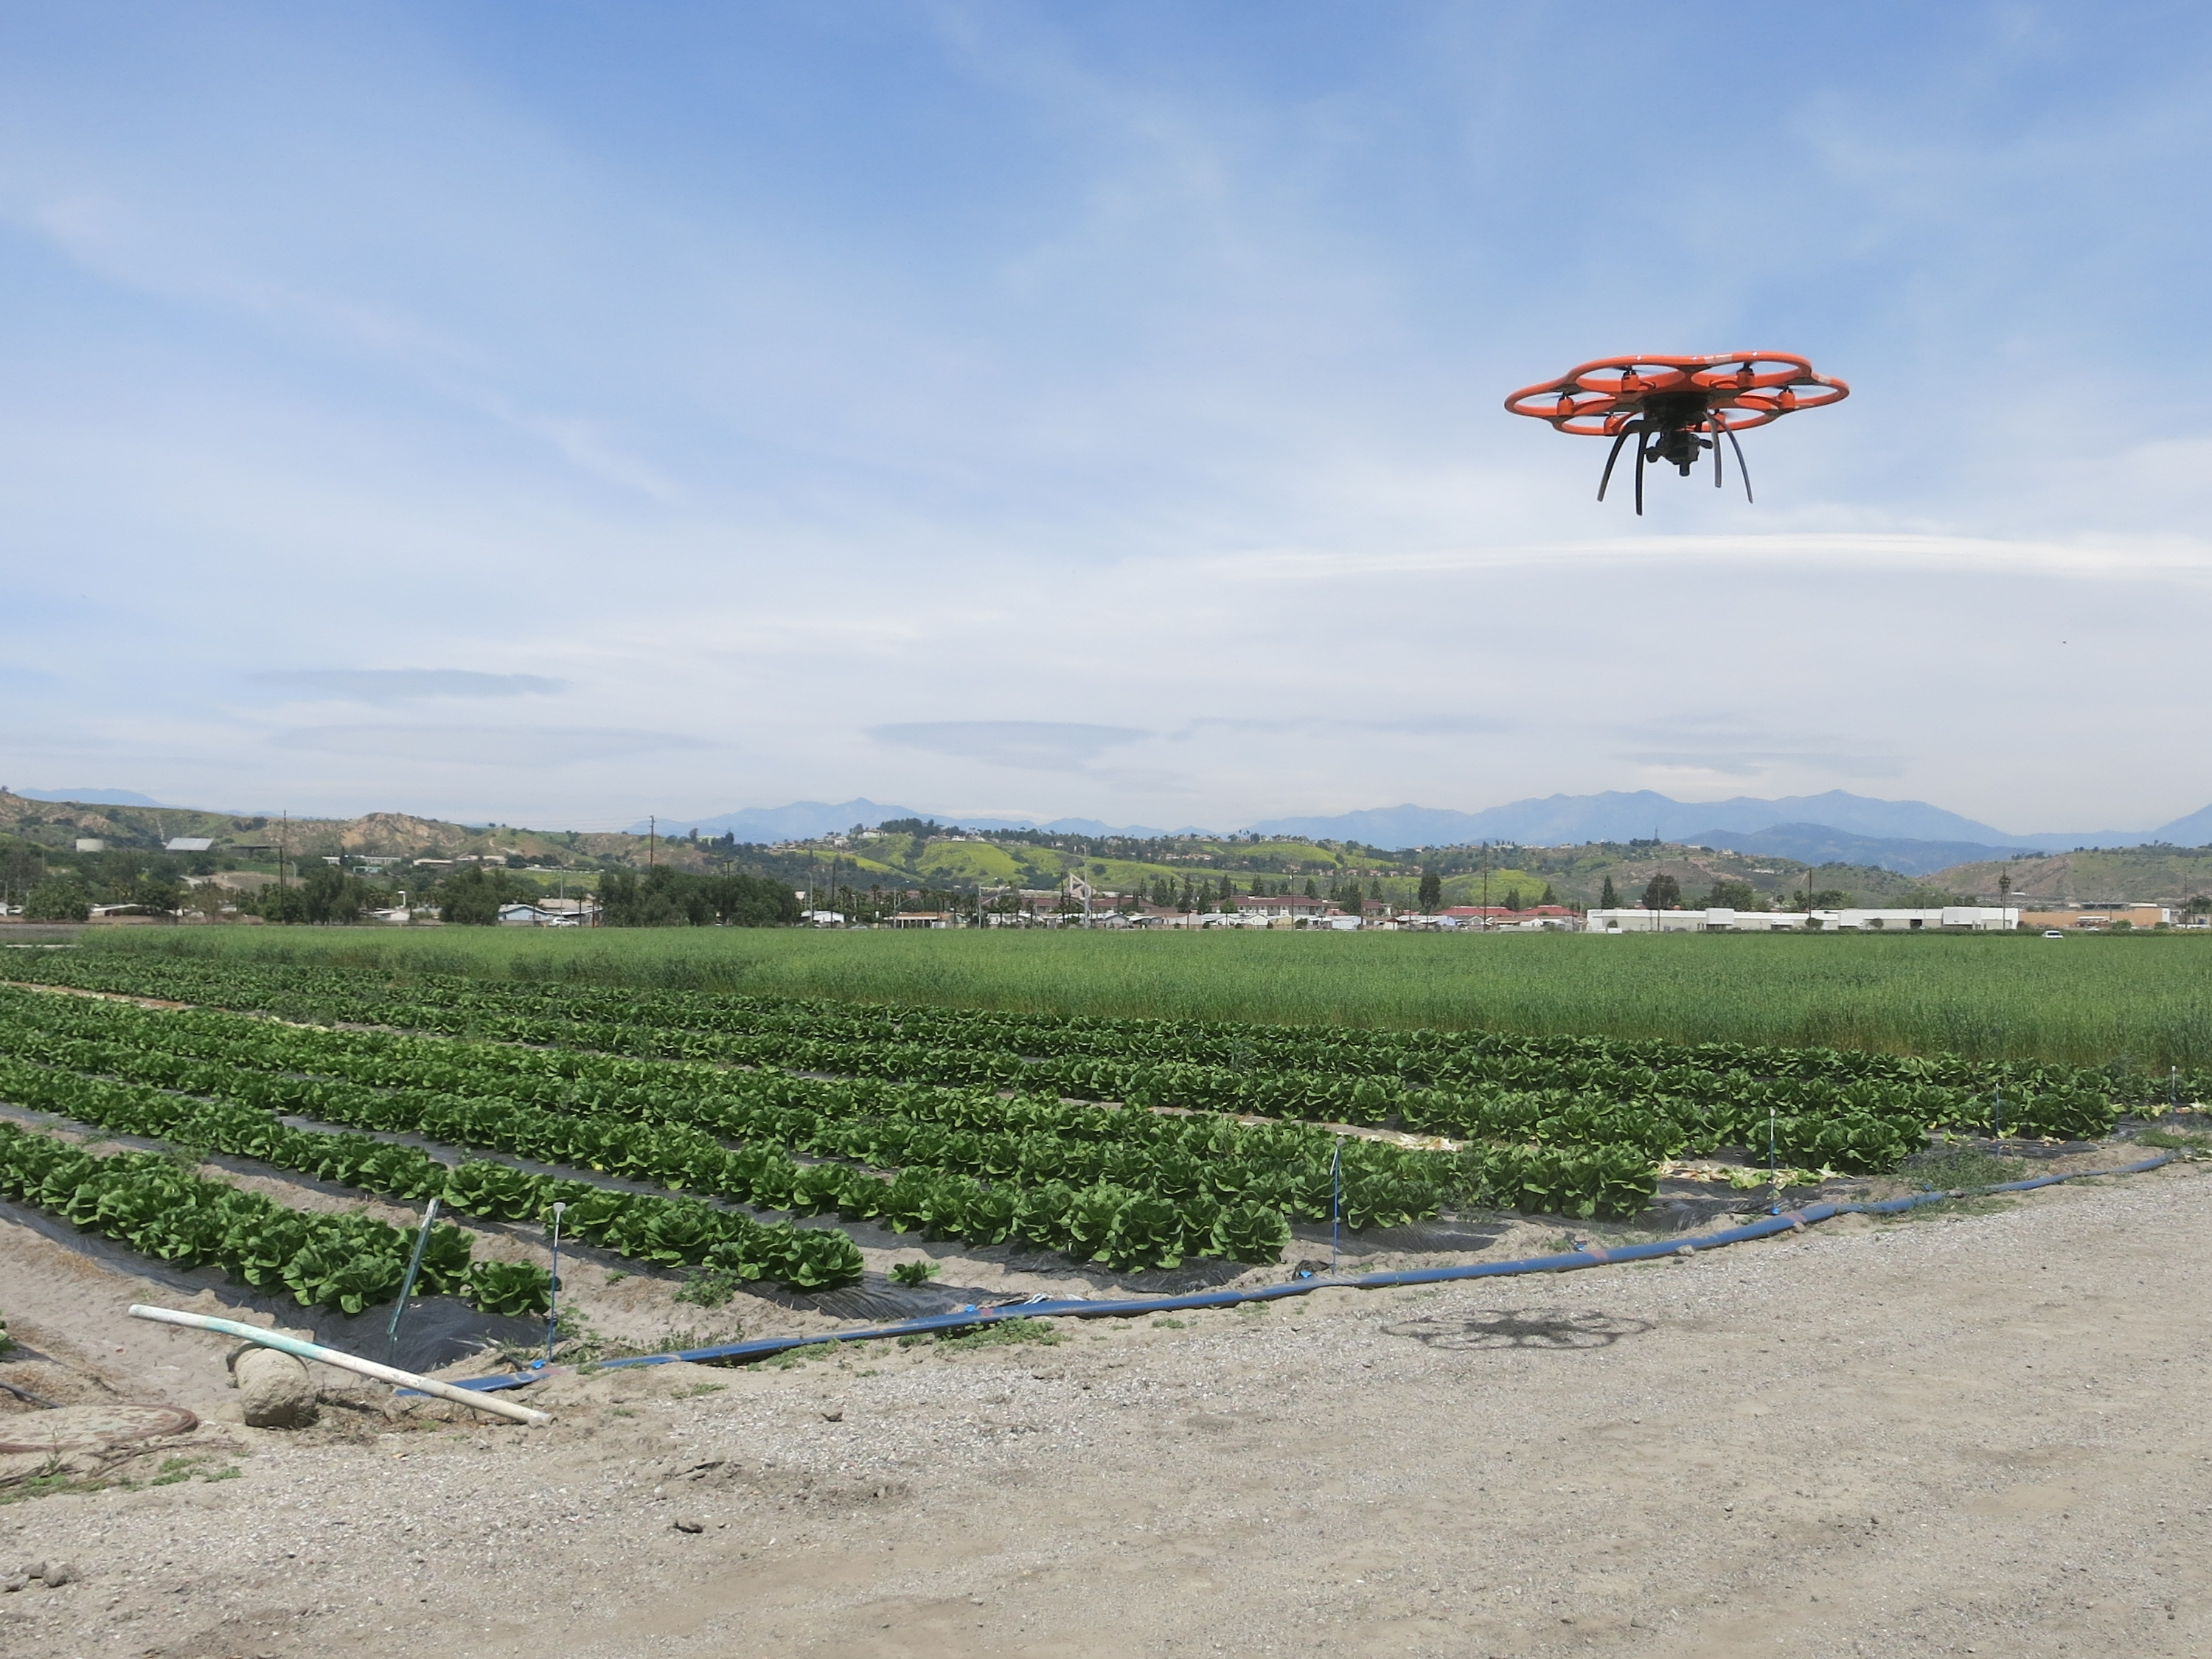
\includegraphics[width=0.8\textwidth]{images/aibotx6.JPG}
    \caption{Aibot X6 from Aibotix collecting data from our lettuce crops.}
    \label{aibotx6}
\end{figure}
\begin{figure}
    \centering
    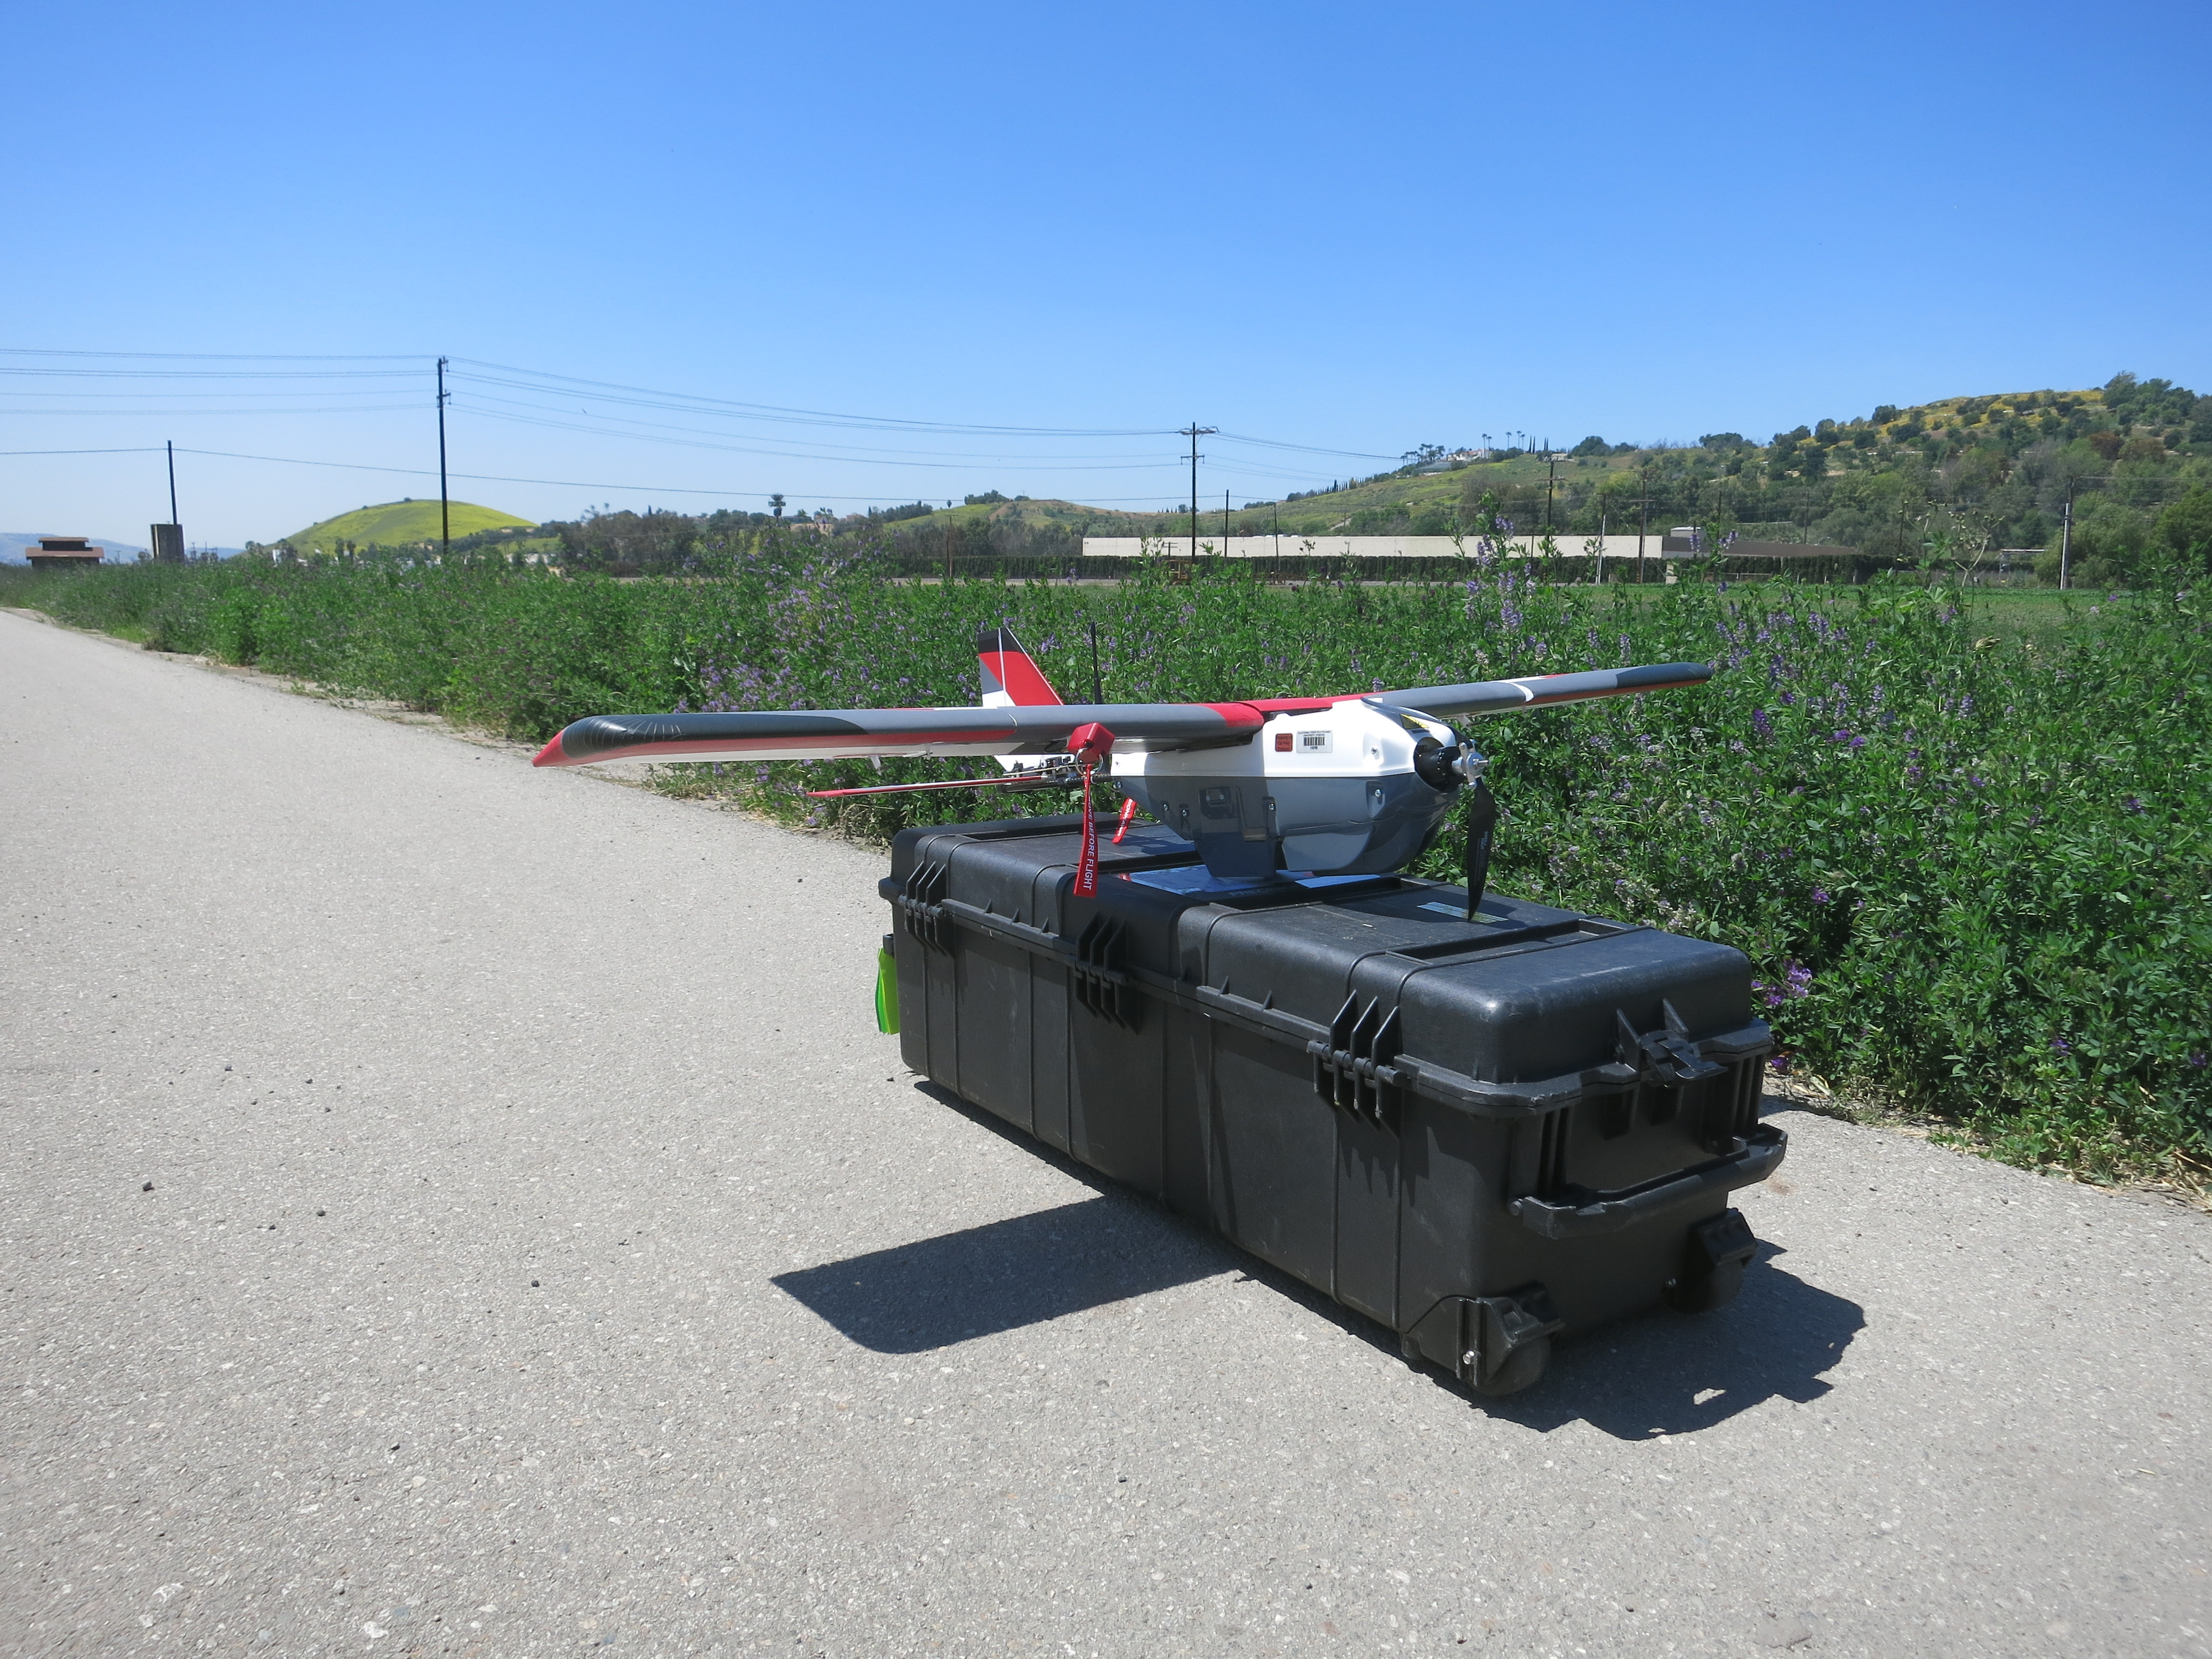
\includegraphics[width=0.8\textwidth]{images/lancaster5.JPG}
    \caption{Lancaster 5 from PrecisionHawk.}
    \label{lancaster5}
\end{figure}

% Spectroradiometer?

To collect chlorophyll data, we used the Konica Minolta SPAD 502. It is a handheld device that measures the amount of chlorophyll in leaves, an indicator of how well fertilized a plant is.

The water potential data was determined using the Decagon WP4C. Leaf cutlets are inserted into the device where the readings are determined. The data is an indicator of how well the plant is being watered.



\subsection{Crop Treatment}
\subsubsection{Lettuce}
The lettuce plants were subjected to 16 different irrigation and nitrogen treatments. The irrigation levels were 0\%, 25\%, 50\% and 100\% of required water according to evapotranspiration. The nitrogen levels were 0\%, 25\%, 50\% and 100\% of required amount for optimal lettuce growth based on soil chemical analysis. This results in the 16 different treatments from the combinations of the 4 levels of irrigation and nitrogen. Each treatment had 3 replications giving us 48 experimental plots as seen in Figure \ref{lettuce_plot}. The treatment was carried out weekly after all the data had been collected.


\begin{figure}
    \centering
    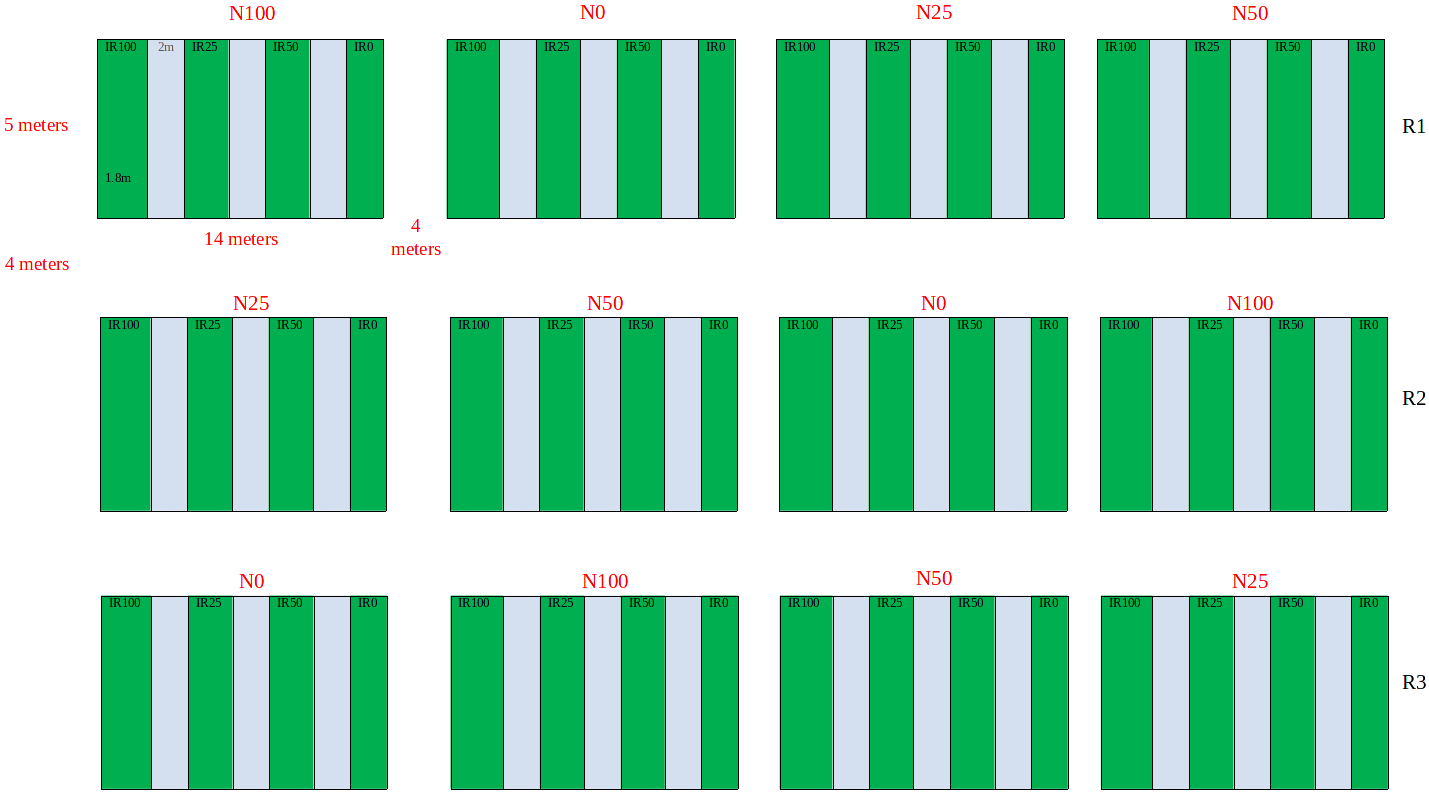
\includegraphics[width=1.0\textwidth]{images/plot.png}
    \caption{Experimental design of lettuce plot.}
    \label{lettuce_plot}
\end{figure}

\subsubsection{Orange Trees}
As the orange trees were planted and maintained by the farm beforehand, we did not implement any treatment plans. The trees followed the treatment that was deemed suitable by the farmers.

\subsection{Data Collection Process}

\subsubsection{Lettuce}
Data was collected weekly at noon as having direct sunlight is optimal for the remote sensing data. 

\subsubsection{Orange Trees}
As with the lettuce, data was also collected weekly at noon.


\section{Models}

\subsection{Predictor}
We utilize a pre-trained Inception network with the final layer removed. We replaced the final layer with the following layers: Dense(512), BatchNormalization, Dropout(0.5), Dense(512), BatchNormalization, Dropout(0.5), Dense(1).

\subsection{Localizer}